\section{Spring MVC}
Nello sviluppo di una API REST tramite Spring Boot è comune l'utilizzo dell'architettura Model-View-Controller(MVC).\\

%\begin{figure}[!h] 
%    \centering 
%    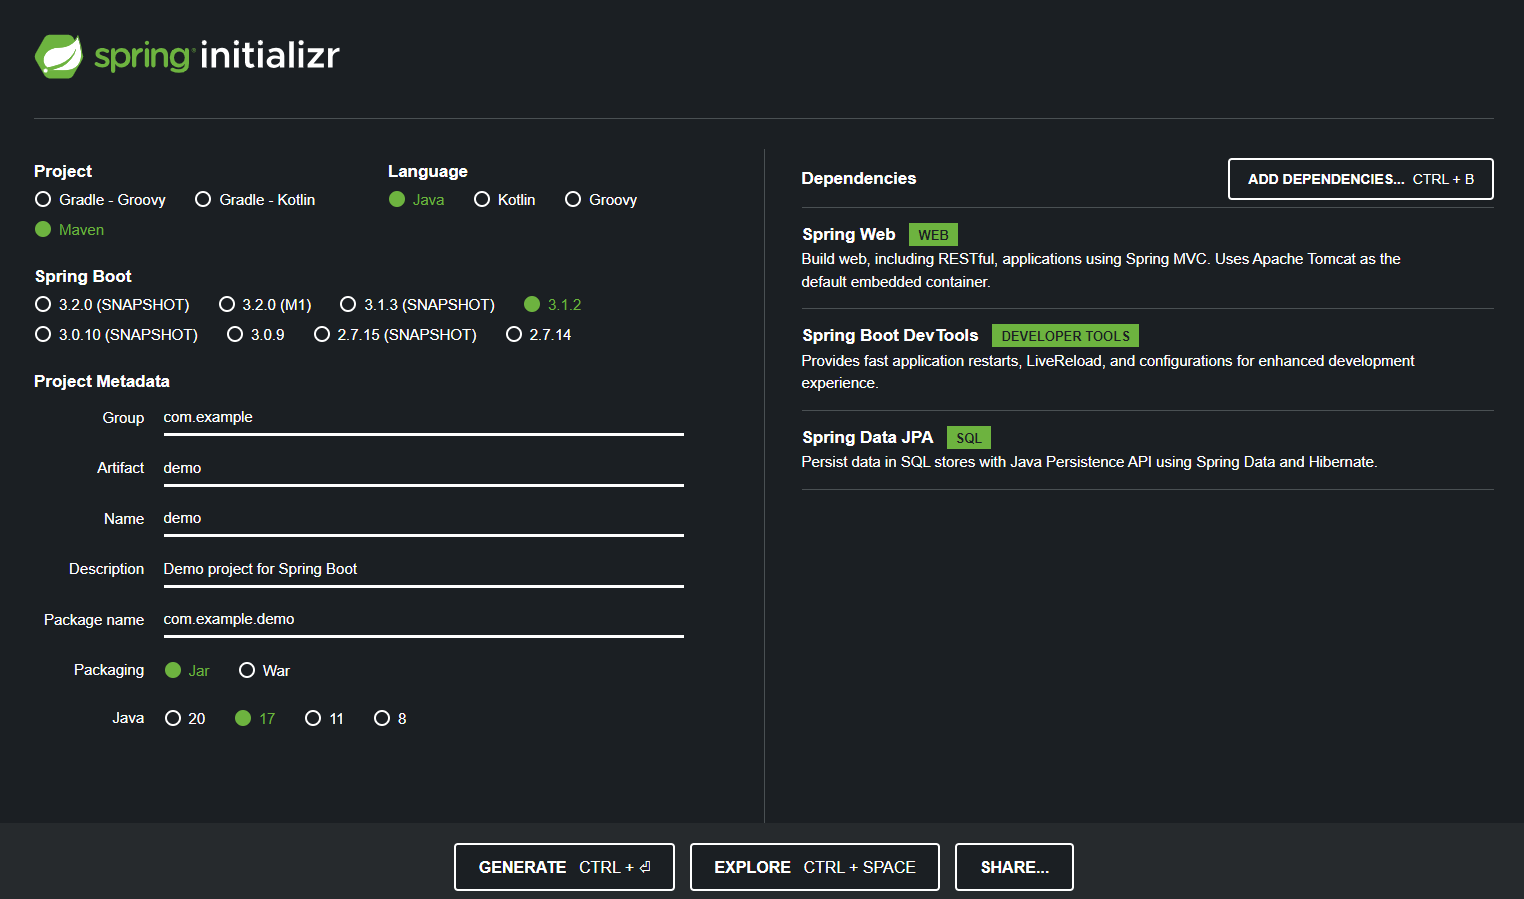
\includegraphics[width=0.95\columnwidth]{Spring_initializr} 
%    \caption{Interfaccia Spring Initializr}
%\end{figure}
\textbf{FOTO MVC}\\

\subsection{Model}
Rappresenta i dati e la business logic\textsubscript{g} dell'applicazione.\\
Nel contesto dello sviluppo di un'API REST, il Model contiene risorse come oggetti di dominio o dati provenienti da una fonte esterna come un database.\\
All'interno del progetto il Model è formato dai seguenti elementi.
\subsubsection{Entità}
In Spring Boot il Model contiene le classi Java segnate con l'annotazione \textit{@Entity} che identifica che quella classe è mappata ad una tabella del database e contiene dati specifici della tabella.
\subsubsection{Repository}
Le repository implementate nel progetto gestiscono l'accesso ai dati e definiscono metodi per eseguire operazioni di base sui dati, come l'inserimento, la modifica, la cancellazione e la ricerca. Tutto questo estendendo interfacce JPA, come \textit{JPARepository}, che consentono di eseguire operazioni in una base di dati senza scrivere codice SQL o query.
\subsubsection{DTO}
Data Transfer Object (DTO), oggetti utilizzati per modellare le rappresentazioni dei dati, utilizzati per definire sia i dati inviati dal client nelle requests che quelli che inviati dal server al cliente nelle responses.

\subsection{View}

\subsection{Controller}

%\begin{itemize}
%\item Entità, corrispondono a classi Java annotate con \textit{@Entity} 
%\end{itemize}
%\subsection*{View}
%dawkodakwpdawdaokdkpaw.\\
%\subsection*{Controller}
%djaopdwkwdkkdw.\\
